\chapter{Related Work}\label{sec:RelatedWork}
Since this is not a novel idea there are some completed solutions and paper written about Fingerprint collection using multiple devices. This chapter will describe few selected solution close to this one for comparison.

\section{Improving Precision by Using Multiple Wearable Devices}\label{sec:IPUMWD}
Focused on improving indoor localization using BLE-based fingerprinting with multiple devices \cite{IPBLEIUMWD}. Using combination of smart phone and wear should in this case prevent signal obstruction from human body and at least one of the devices should receive beacon signal. Unfortunately due to low BLE sensibility of wear devices, authors decided to supplement them with smartphone, in this case with Nexus 5 running Android 4.4.

This paper proposes calculating medians using 800 millisecond tests where user can move at most one meter. For all medians at the same position is calculated average and variance, based on which a normal distribution is used to model the potential variation of RSSI. One thing to note is that fingerprint maps are built based on facing direction. There are five main scenarios tested

\begin{itemize}
	\item P1: device held in hand where body does not obstruct its LOS path to all beacons,
	\item P2: device is put in breast pocket and LOS may be obstructed to some beacons,
	\item P3: user holds smartphone in hand and wears a smartwatch on one wrist,
	\item P4: one device is put in the breast pocket and the other is on one wrist,
	\item P5: one device is in the breast pocket, and two other devices, each on one wrist.
\end{itemize} 

Firstly, four of these scenarios were tested in a 15x8 meters entrance hall with four deployed beacons in the corners and ten measurement positions. In this location using multiple devices can improve position precision and reduce error by 57\%. \tref{tab1} shows mean errors for previously mentioned cases where using more devices improves localization. However there is one position where case P4 will result with higher error then P3 due to building structure and signal obstruction for nearest beacons.

\begin{table}[h]
	\begin{center}
			\begin{tabular}{| l | c |}
				\hline
				Scenario & Mean error (m) \\ \hline
				P1 & 2.36 \\
				P2 & 1.71 \\
				P3 & 0.96 \\
				P4 & 0.41 \\ \hline
		\end{tabular}
		\caption{Mean errors at first location (sources: \cite{IPBLEIUMWD})}
		\label{tab1}
	\end{center}
\end{table} 

Secondly, all of previously mentioned scenarios were tested in a conference room with unified ceiling and desks near the walls. This location is used to investigate the impact of beacon density to position precision. Three following combinations of beacons are used

\begin{itemize}
	\item A: four beacons at the corners,
	\item B: combination A with one beacon at the center,
	\item C: combination B with four more beacons at the sides of the room.
\end{itemize}

Using directional maps at this location resulted in increase of maximum localization error, which was not expected. This error can increase even more when using higher count of beacons and occurs mostly when testing at the edges of the room. Mean error on the other hand shows an improvement, higher with more beacons used. 

\begin{table}[h]
	\begin{center}
			\begin{tabular}{ | l | c c c | }
				\hline
				 & \multicolumn{3}{ c | }{Mean error (m)} \\ \hline
				Scenario & A & B & C \\ \hline
				P1 & 2.05 & 2.05 & 1.76 \\ 
				P2 & 1.84 & 1.49 & 0.90 \\ 
				P3 & 1.36 & 1.09 & 0.63 \\ 
				P4 & 1.24 & 0.78 & 0.23 \\ 
				P5 & 0.80 & 0.39 & 0.07 \\ \hline
		\end{tabular}
		\caption{Mean errors at second location (sources: \cite{IPBLEIUMWD})}
		\label{tab2}
	\end{center}
\end{table} 

In summary, position error can be improved by three aspects: using more devices, using directional map or increasing the number of beacons. There are two main conclusions of this paper. First, confirmed precision degradation when testing near the edge of the room with obstructed signal from nearest beacon. Second, human body does not greatly change radio signal and device can receive reflected signals with sufficient strength. 

\section{SmartFix}\label{sec:SmartFix}
An Indoor Locating Optimization Algorithm for Energy-Constrained Wearable Devices called SmartFix \cite{SmartFix}. The main goal of this paper is improve energy consumption efficiency for wearable-based indoor localization using WiFi fingerprints. Single real-time experiment of energy consumption was run and split into two main parts: computation of location and collection of fingerprints. According to this experiment, energy consumption caused by collection is occupies 99\% of localization algorithm.

This paper proposes novel indoor localization strategy, SmartFix, that can cooperate with existing indoor localization technologies based on WiFi. It enhances accuracy of such algorithm with a little extra energy cost of calculation but a large save of signal collection energy cost. Aided with machine-learning algorithm, it obtains the relative features given the trajectories of users in certain areas and modify the localization results. SmartFix can save up to 70\% of energy while achieving the same localization accuracy when compared to the original fingerprint method.

To test this new system it was implemented with prototypes of TinyLoc \cite{TinyLoc}, MoLoc \cite{MoLoc} and basic WiFi fingerprint method using k-neighbor algorithm. TinyLoc is more focused on energy efficiency than location accuracy. In contrast SmartFix analyses the history trajectory of people in given area to improve locating results. It refers to user motion features, SmartFix modifies locating results to achieve satisfying accuracy. MoLoc also leverages user motion by collecting trajectory patterns using device built-in sensors.

All previously mentioned prototypes were deployed with and without SmartFix to test its power consumptions. It only needs single real-time RSS signal in the
locating phase to guarantee excellent energy saving performance. \fref{fig6} shows energy consumption of on-time locating on two specific devices: HTC one and Moto 360. 

\begin{figure}[H]
	\begin{centering}
		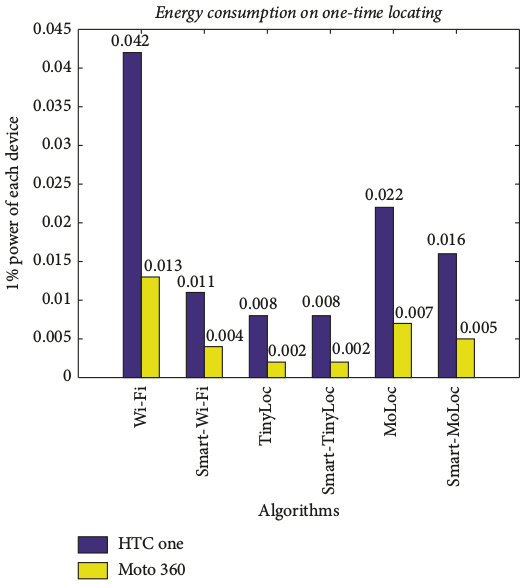
\includegraphics[width=0.6\textwidth]{img/smart_fix}
		\par\end{centering}
	\caption{Energy consumption based on prototypes (source: \cite{SmartFix})\label{fig:SmartFix}}
	\label{fig6}
\end{figure}

This paper proposed an tested new localization technology, SmartFix, which main focus is to improve energy efficiency for wearable devices. According to experiment, the probability of error within 2 meter can be reached in 80\% of cases. Meanwhile, energy consumption is 35\% lower than that of MoLoc with the same accuracy, and SmartFix obtains best accuracy with minimal energy cost.

\section{SmartWatch vs. SmartPhone}\label{sec:SWvsSP}

http://www.eislab.fim.uni-passau.de/files/publications/2017/1570325956.pdf
